\documentclass[11pt,landscape,a4paper]{article}
\usepackage[utf8]{inputenc}
\usepackage[ngerman]{babel}
\usepackage[T1]{fontenc}
%\usepackage[LY1,T1]{fontenc}
%\usepackage{frutigernext}
%\usepackage[lf,minionint]{MinionPro}
\usepackage{tikz}
\usetikzlibrary{shapes,positioning,arrows,fit,calc,graphs,graphs.standard}
\usepackage[nosf]{kpfonts}
\usepackage[t1]{sourcesanspro}
\usepackage{multicol}
\usepackage{wrapfig}
\usepackage[top=4mm,bottom=4mm,left=4mm,right=4mm]{geometry}
\usepackage[framemethod=tikz]{mdframed}
\usepackage{microtype}
\usepackage{pdfpages}
\usepackage[shortlabels]{enumitem}
\usepackage{flushend}
\usepackage{physics}
\usepackage{listings}
\usepackage{bbding}

\raggedend 

\newif\iflong
\longtrue % \longfalse for short version and \longtrue for long version
\newcommand{\inLongVersion}[1]{\iflong #1\fi}


\setlist{nosep}
\setlist[itemize]{leftmargin=*}
\setlist[enumerate]{leftmargin=*}

\newcommand{\score}{\text{score}}
\newcommand{\encoder}{\text{encoder}}
\newcommand{\decoder}{\text{decoder}}
\newcommand{\E}{\mathbb{E}}
\newcommand{\Dist}{\mathcal{D}}
\newcommand{\normal}{\mathcal{N}}
\DeclareMathOperator{\cov}{\textbf{Cov}}
% \DeclareMathOperator{\var}{\textbf{Var}}
\DeclareMathOperator{\argmin}{\textbf{argmin}}
\DeclareMathOperator{\argmax}{\textbf{argmax}}
\DeclareMathOperator{\sgn}{\textbf{sgn}}
\DeclareMathOperator{\dir}{\textbf{Dir}}
\DeclareMathOperator{\cat}{\textbf{Cat}}
\DeclareMathOperator{\KL}{\mathsf{KL}}
\DeclareMathOperator{\JS}{\mathsf{JS}}


\let\bar\overline

\definecolor{myblue}{cmyk}{0,0,0,1}


\def\firstcircle{(0,0) circle (1.5cm)}
\def\secondcircle{(0:2cm) circle (1.5cm)}

\colorlet{circle edge}{myblue}
\colorlet{circle area}{myblue!5}

\tikzset{filled/.style={fill=circle area, draw=circle edge, thick},
    outline/.style={draw=circle edge, thick}}
    
\pgfdeclarelayer{background}
\pgfsetlayers{background,main}

\everymath\expandafter{\the\everymath \color{myblue}}
\everydisplay\expandafter{\the\everydisplay \color{myblue}}

\renewcommand{\baselinestretch}{.8}
\pagestyle{empty}

\global\mdfdefinestyle{header}{%
linecolor=gray,linewidth=1pt,%
leftmargin=0mm,rightmargin=0mm,skipbelow=0mm,skipabove=0mm,
}

\newcommand{\header}{
\begin{mdframed}[style=header]
\footnotesize
\sffamily
\centering
AML, Yuhao Mao,~Page~\thepage
\end{mdframed}
}

\makeatletter % Author: https://tex.stackexchange.com/questions/218587/how-to-set-one-header-for-each-page-using-multicols
\renewcommand{\section}{\@startsection{section}{1}{0mm}%
                                {.5ex}%
                                {.5ex}%x
                                {\color{myblue}\sffamily\bfseries}}
\renewcommand{\subsection}{\@startsection{subsection}{2}{0mm}%
                                {.2ex}%
                                {.2ex}%x
                                {\sffamily\bfseries}}
\renewcommand{\subsubsection}{\@startsection{subsubsection}{3}{0mm}%
                                {.1ex}%
                                {.1ex}%x
                                {\sffamily\itshape}}



\def\multi@column@out{%
   \ifnum\outputpenalty <-\@M
   \speci@ls \else
   \ifvoid\colbreak@box\else
     \mult@info\@ne{Re-adding forced
               break(s) for splitting}%
     \setbox\@cclv\vbox{%
        \unvbox\colbreak@box
        \penalty-\@Mv\unvbox\@cclv}%
   \fi
   \splittopskip\topskip
   \splitmaxdepth\maxdepth
   \dimen@\@colroom
   \divide\skip\footins\col@number
   \ifvoid\footins \else
      \leave@mult@footins
   \fi
   \let\ifshr@kingsaved\ifshr@king
   \ifvbox \@kludgeins
     \advance \dimen@ -\ht\@kludgeins
     \ifdim \wd\@kludgeins>\z@
        \shr@nkingtrue
     \fi
   \fi
   \process@cols\mult@gfirstbox{%
%%%%% START CHANGE
% \ifnum\count@=\numexpr\mult@rightbox+2\relax
%           \setbox\count@\vsplit\@cclv to \dimexpr \dimen@-1cm\relax
% \setbox\count@\vbox to \dimen@{\vbox to 1cm{\header}\unvbox\count@\vss}%
% \else
%       \setbox\count@\vsplit\@cclv to \dimen@
% \fi
\setbox\count@\vsplit\@cclv to \dimen@
%%%%% END CHANGE
            \set@keptmarks
            \setbox\count@
                 \vbox to\dimen@
                  {\unvbox\count@
                   \remove@discardable@items
                   \ifshr@nking\vfill\fi}%
           }%
   \setbox\mult@rightbox
       \vsplit\@cclv to\dimen@
   \set@keptmarks
   \setbox\mult@rightbox\vbox to\dimen@
          {\unvbox\mult@rightbox
           \remove@discardable@items
           \ifshr@nking\vfill\fi}%
   \let\ifshr@king\ifshr@kingsaved
   \ifvoid\@cclv \else
       \unvbox\@cclv
       \ifnum\outputpenalty=\@M
       \else
          \penalty\outputpenalty
       \fi
       \ifvoid\footins\else
         \PackageWarning{multicol}%
          {I moved some lines to
           the next page.\MessageBreak
           Footnotes on page
           \thepage\space might be wrong}%
       \fi
       \ifnum \c@tracingmulticols>\thr@@
                    \hrule\allowbreak \fi
   \fi
   \ifx\@empty\kept@firstmark
      \let\firstmark\kept@topmark
      \let\botmark\kept@topmark
   \else
      \let\firstmark\kept@firstmark
      \let\botmark\kept@botmark
   \fi
   \let\topmark\kept@topmark
   \mult@info\tw@
        {Use kept top mark:\MessageBreak
          \meaning\kept@topmark
         \MessageBreak
         Use kept first mark:\MessageBreak
          \meaning\kept@firstmark
        \MessageBreak
         Use kept bot mark:\MessageBreak
          \meaning\kept@botmark
        \MessageBreak
         Produce first mark:\MessageBreak
          \meaning\firstmark
        \MessageBreak
        Produce bot mark:\MessageBreak
          \meaning\botmark
         \@gobbletwo}%
   \setbox\@cclv\vbox{\unvbox\partial@page
                      \page@sofar}%
   \@makecol\@outputpage
     \global\let\kept@topmark\botmark
     \global\let\kept@firstmark\@empty
     \global\let\kept@botmark\@empty
     \mult@info\tw@
        {(Re)Init top mark:\MessageBreak
         \meaning\kept@topmark
         \@gobbletwo}%
   \global\@colroom\@colht
   \global \@mparbottom \z@
   \process@deferreds
   \@whilesw\if@fcolmade\fi{\@outputpage
      \global\@colroom\@colht
      \process@deferreds}%
   \mult@info\@ne
     {Colroom:\MessageBreak
      \the\@colht\space
              after float space removed
              = \the\@colroom \@gobble}%
    \set@mult@vsize \global
  \fi}

\makeatother
\setlength{\parindent}{0pt}




\begin{document}
%\footnotesize
\small

    \begin{sectionbox}{pink}\section{Introduction}
\textbf{MLE}: \(\hat{\theta} = \arg\max_\theta \sum_{i}\log p(x_i|\theta)\).

\textbf{MLPs are universal function approximators} / Boolean machines / classification functions: $\sigma$ non-constant bounded continuous, $\epsilon > 0$, $\forall f \in C(I_m)$ (cube of dim m), $f(x) \approx g(x) = \sum_{i=1}^{n} v_i \sigma(w_i^T x + b_i)$ (single hidden layer).

\textbf{Double Descent} both epoch-wise and model complexity-wise: bias-variance tradeoff until interpolation threshold, then gets better again. $\text{EMC}_{D,\epsilon}(\mathcal{T}) = \max\{n | \mathbb{E}_{S\sim D}\left[\text{Error}_S(\mathcal{T}(S))\right] \leq \epsilon\}$. If $\ll n$ (underparam) or $\gg n$ (overparam) can decrease test error by making $n$ bigger, if $\approx n$ error can increase or decrease.

\textbf{Supervised learning} \(f\) maps data \(x\to\) label \(y\).
\textbf{Unsupervised learning} data underlying structure: clustering, feature learning, dim reduction, density estimation.

\textbf{Generative modelling} learn \(p_{\text{M}}\) sim to \(p_{\mathcal{D}}\), then sample from\(p_{\text{M}}\):
\begin{itemize}
    \item Explicit density: \begin{itemize}
        \item Approximate: \begin{itemize}
            \item Variational: VAE, Diffusion
            \item \textcolor{gray}{Markov Chain: Boltzmann mach.}
        \end{itemize}
        \item Tractable: \begin{itemize}
            \item Autoregressive: FVSBN/NADE/MADE, Pixel(c/r)nn, WaveNet/tcn, Autoregressive Transformer, LLM
            \item Normalizing Flows
        \end{itemize}
    \end{itemize}
    \item Implicit density: \begin{itemize}
        \item Direct: Generative Adversarial Nets
        \item \textcolor{gray}{Markov Chain: Gen Stoch Nets}
    \end{itemize}
\end{itemize}\end{sectionbox}
\begin{sectionbox}{blue}\section{CNN}

\textbf{Neural Findings}
(1) Rapid serial visual presentation(RSVP), (2) Hubel \& Wiesel, receptive fields (3) HMAX Model, simple/complex cell.

\textbf{Pre-DL Model}: Neurocognitron, LeNet-5, \textbf{Dataset}: ImageNet challenge.

\textbf{3 Properties}:\\
(1) \textbf{Linear} \(T(\alpha {u}+\beta {v})=\alpha T({u})+\beta T({v})\).\\ (2) \textbf{Invariance} to \(f\), \(T(f({u}))=T({u})\).\\ (3) \textbf{Equivariance} to \(f\), \(T(f({u}))=f(T({u}))\).

\subsection*{Convolution}
\textbf{Correlation} $A \otimes B$ \hspace{\stretch{1}} \textbf{Convolution} $A \ast B$
(Cross-)Correlat. slides matrices in original orientation, and $A \ast B = A \otimes \text{ROT}_{180^{\circ}}(B)$



\textsf{F}:\( z_{ij}^{(l)}=w^{(l)} * z^{(l-1)}+b= \sum_{mn} w_{mn}^{(l)} z_{i-m, j-n}^{(l-1)}+b\). \\
\textsf{B} on \(z\):\(\delta_{i,j}^{(l-1)} := \pdv{C}{z^{(l-1)}_{i,j}} = \sum_{i'j'} \pdv{C}{z^{(l)}_{i,j}} \pdv{z^{(l)}_{ij}}{z^{(l-1)}_{ij}} =  \sum_{i'j'} \delta_{ij}^{(l)} w_{i'-l,j'-j}^{(l)} = \delta^{(l)} * \text{ROT}_{180^{\circ}}(w^{(l)})\).\\
\textsf{B} on \(w\):\(\pdv{C}{w^{(l)}_{m,n}} =  \sum_{i',j'} \pdv{C}{z^{(l)}_{i,j}} \pdv{z^{(l)}_{i,j}}{w^{(l)}_{m,n}} =  \delta^{(l)} * \text{ROT}_{180^{\circ}}(z^{(l-1)})\)

\( L_{\text{out}}=\left\lfloor \frac{  L_{\text{in}} + 2\text{Pad}_{=0} - \text {Dilat}_{=1}(\text{Ker} - 1)-1 }{\text {Stride}_{=1}} + 1 \right\rfloor \) for \verb|Conv| and \verb|Pool|.

\(n_{\text{connect}}\) of each neuron \(3k^2\).\\
\(n_{\text{para}} = ( k^2 \text{dim}_{\text{in}} + 1)\text{dim}_{\text{out}}\)

Correlation \(\Leftrightarrow\) \verb|Conv| only \(C_{m,n} = K_{-m,-n}\).

\verb|Conv| can be seen as Matmul, \(I * K = \mathsf{K I}\),
% \begin{footnotesize}
%     \begin{equation*}
%         I * K = \left(\begin{array}{ccc}
%             k_{1} & 0             & 0      \\
%             k_{2} & k_{1}         & \vdots \\
%             0     & k_{2}         & \vdots \\
%             0     & \vdots \cdots & k_{m}
%         \end{array}\right) \left(\begin{array}{c}
%             I_{1}  \\
%             \vdots \\
%             I_{n}
%         \end{array}\right)
%     \end{equation*}
% \end{footnotesize}

Differentiation by \verb|Conv|, \(\text{Ker} = (1, -1)\).

Weight sharing btw pixels.

\subsection*{Pooling}
\textbf{Goal} (1) increase receptive field. (2) noise robustness. \\
\textbf{Max-Pool} \textsf{F}: \(z^{(l)}=\max \{z_{i}^{(l-1)}\}\), \textsf{B}: \(\delta^{(l-1)}=\{\delta^{(l)}\}_{i^{*}=\operatorname{argmax}_{i}\{z_{i}^{(l-1)}\}}\).

\subsection*{Application}
\textbf{Alexnet} Smaller filter, more layers. \\
\textbf{VGG} +layers, -params, +receptive field. \\
\textbf{GoogLeNet} Deeper, Inception module, 1x1 conv for dim/channel reduction\(64\to 32\), Auxiliary \verb|cls| head \(\Rightarrow\) More efficient. \\
\textbf{ResNet} +layers, faster, uses residual connections: (1) better convergence. (2) propagate high freq info (U-net).\\
\textbf{U-Net} fully CNN, combine global+local features using tensors from prev layer.

\subsection*{Fully CNN}

CNN + final MLP only fixed size, for segmentat. can't see whole context; fully CNN convolutions at original image size expensive so uses down+up-sampling.

\textbf{Unpooling Methods}: Nearest Neighbor, Bed of Nail, Max Unpooling (need maxpool from prev net).

\textbf{ConvTranspose2D / strided upconvolution} shape: \(L_{\text{out}} = (L_{\text{in}} - 1)\text{Stride}_{=1} - 2  \text{Pad}_{=0} + \text{Dilat}_{=1}(\text{Ker} - 1) + \text{OutPad}_{=0} + 1\)

Motion infilling uses conv. autoenc.\end{sectionbox}
% \begin{sectionbox}{olive}\section{Full CNN, upsampling}
\textbf{Goal} Pixel predict, semantic seg.

\textbf{Unpooling Methods}: Nearest Neighbor, Bed of Nail, Max Unpooling (need maxpool from prev net).

\subsection*{ConvTranspose2D}
\textbf{shape}: \(L_{\text{out}} = (L_{\text{in}} - 1)\text{Stride}_{=1} - 2  \text{Pad}_{=0} + \text{Dilat}_{=1}(\text{Ker} - 1) + \text{OutPad}_{=0} + 1\)

\textbf{App} U-Net: combine global+local features using tensors from previous layer.

\end{sectionbox}
\begin{sectionbox}{magenta}\section{RNN}
\textbf{Def} \(h^{t}=f(h^{t-1}, x^{t} ; W), \hat{y}^{t}=W_{h y} h^{t}\).\\ Loss \(L = \sum_t L^{t} =\sum_t L(y^{t}, \hat{y}^{t})\).

\textbf{BPTT} \(\frac{\partial L^{t}}{\partial W}=\sum_{k=1}^{t} \frac{\partial L^{t}}{\partial \hat{y}^{t}} \frac{\partial \hat{y}^{t}}{\partial h^{t}} \frac{\partial h^{t}}{\partial h^{k}} \frac{\partial^{+} h^{k}}{\partial W}\),\\
\(\frac{\partial h^{t}}{\partial h^{k}}=\prod_{i=k+1}^{t} W_{h}^{T} \operatorname{diag}[f^{\prime}(h^{i-1})]\).


\subsection*{Gradient vanishing/exploding}
\(\lambda_1 := \max \lambda(W_{hh})\), \(\gamma > \|\operatorname{diag}(f^{\prime}(h^{i-1}))\|\), then \(\lambda_1 \gtrless  \gamma^{-1}\) vanish/explode.

\textbf{DisAdv for GV/E} (1) Instabilities during training lead to Inf/NaN. (2) hard to capture long-term dependencies, cuz no gradient at lower levels, no learning. (3) large gradients\(\Leftrightarrow\)jumper over local minima or oscillate.

\textbf{Gradient clipping}\(\to\)prevent \(\nabla\) explode.

\textbf{LSTM} Inpt, forgt, outpt \(\in [0, 1]\), gate \(\in\mathbb{R}\).

(predecessor to LSTM is GRU)

\textbf{Vanila}: \(h_{t}=\tanh W\left(\begin{array}{l}
    x_t \\
    h_{t-1}
    \end{array}\right)\).
\textbf{LSTM}:

\(\left(\begin{array}{l}
    i \\
    f \\
    o \\
    g
    \end{array}\right)=\left(\begin{array}{c}
    \operatorname{sigm} \\
    \operatorname{sigm} \\
    \operatorname{sigm} \\
    \tanh
    \end{array}\right) W\left(\begin{array}{l}
    x_t \\
    h_{t-1}
    \end{array}\right)\),
\(W : 4 n \!\!\times\!\! 2 n\), \(c_{t}=f \odot c_{t-1}+i \odot g\) \hspace{\stretch{1}} \(h_{t}=o \odot \tanh (c_{t})\)
\end{sectionbox}
\begin{sectionbox}{lime}\section{Variational Auto-Encoder}

\subsection*{Auto-Encoder (AE)}

\textbf{Encoder} proj to latent space $z$, \textbf{Decoder} proj back. \textbf{Loss} \(\sum ||x_i - g(f(x_i))||_2^2\).
Optimal linear autoencoder is PCA. Undercomplete: $|Z| < |X|$, else overcomplete. Overcomp. is for denoising, inpainting.

\textbf{Dis/Adv} Reconstruction \Checkmark, Generation \XSolidBrush. Latent space not well-structured: no continuity, no interpolation.

\textbf{Applications} (1) Denoising AE: randomly set pixels to 0 then recover. (2) Inpainting AE: cover part of image then recover. (3) 3D Human Motion: add noise to skeleton, recover with AE then pass to LSTM per frame.



\subsection*{Variational Auto-Encoder (VAE)}
\begin{small}
\(\ln p_{\theta}({x}) = \operatorname{ELBO}_{\theta, \phi}({x}) + \KL(q_{\phi}(z | {x}) \| p_{\theta}(z | {x}))\). \\
Objective: \(\max_{\theta, \phi} \sum_i \operatorname{ELBO}_{\theta, \phi}({x_i})\).\\
\( \operatorname{ELBO}= \mathbb{E}_{q_{\phi}}\ln p_{\theta}(x | z) - \KL (q_{\phi}(z | x)|| p_{\theta}(z))\)
\end{small}


\(\mathbb{E}_{q_{\phi}}[\log p_{\theta}(x | z)]\) reconstruction likelihood, encourage clustering for similar samples in latent space. \(-\KL(q_{\phi}(z | x)|| p_{\theta}(z))\) makes posterior close to prior, encourages latent representations evenly around center, compactness, smooth interp.

(1) If only recon: VAE\(\to\)AE, sharp recon but sparce latent space. (2) No recon loss: compact embedding like Gaussian, but bad for reconstruction.

Encoder: \(q_{\phi}(z | x) = \mathcal{N}(\mu_{\mathsf{nn}}(x), \Sigma_{\mathsf{nn}}(x))\), \\
Decoder: \(p_{\theta}(x | z) = \mathcal{N}(\mu_{\mathsf{nn}}(z), \Sigma_{\mathsf{nn}}(z))\).

Approximate $\mathbb{E}$ in loss with sampling.

\begin{small}
\textbf{Derivation} \(\log{p(x)} = \log \int p(z) p(x|z) \,dz    = \log \int p(z) p(x|z) \frac{q(z|x)}{q(z|x)} \,dz    = \log \mathbb{E}_{z \sim q(z|x)}\left[p(x|z) \frac{p(z)}{q(z|x)}\right]    \geq \mathbb{E}_{z \sim q(z|x)}\left[\log \left(p(x|z) \frac{p(z)}{q(z|x)}\right)\right]    = \mathbb{E}_{z \sim q(z|x)}\left[\log p(x|z) - \log \frac{q(z|x)}{p(z)}\right]    =\mathbb{E}_{z \sim q(z|x)}\left[\log p(x|z)\right] - D_{\text{KL}} (q(z|x) | | p(z))\)
\end{small}

% Example: MNIST, Facial expression.

\subsection*{Disentangle respresentation}
\textbf{semi-super}v-learn can lead to disentangle. \(p(x|y, z)\), \(y\) digits, \(z\) style. \\
\textbf{UnSuper}vised disentangle, \(\beta\)-\textbf{VAE}: \\
Assume \(p({x} | {z}) \approx p({x} | {v}, {w})\), \(v\) conditionally indep factors, \(w\) cond dep facts (entangled), \(\log p({v} | {x}) = \sum_{k} \log p(v_{k} | {x})\). Train:
\(\max _{\phi, \theta} \mathbb{E}_{x,q_{\phi}} \ln p_{\theta}(x | z)\), s.t. \(\KL(q_{\phi} \| p_{\theta}(z))\) \(<\delta\Leftrightarrow L_{\beta,\phi,\theta}=\mathsf{NLL}+\beta \KL\), \(\beta > 1\) stronger constraint on latent space than VAE.


\subsection*{Hierarchical Latent Variable Models}
Encoder \(q_{\phi}(z_{1:L}| x)= \prod_{i=1}^{L}q_{\phi}(z_{i} | x) \),
Decoder  \(p_{\theta}(x|z) = p_{\theta}(x|z_1)\),
Prior \(p_{\theta}(z_{1:L})=p_{\theta}(z_{L}) \prod_{i=1}^{L-1} p_{\theta}(z_{i} | z_{i+1})\),
\(\mathcal{L}_{\theta, \phi}(x)=\mathbb{E}_{q_{\phi}}[\log p_{\theta}(x | z_{1})]-D_{K L}(q_{\phi}(z_{L} | x) \| p_{\theta}(z_{L}))-\sum_{i=1}^{L-1} \mathbb{E}_{z_{i+1} \sim q_{\phi}(z_{i+1} | x)} D_{K L}(q_{\phi}(z_{i} | x) \| p_{\theta}(z_{i} | z_{i+1}))\).
\end{sectionbox}
\begin{sectionbox}{violet}\section{Autoregressive models}
\textbf{Goal} Density estim \(p({x}) = \prod_{i} p({x}_{i} | {x}_{<i})\).

\subsection*{Fully Visible Sigmoid Belief Networks}

Tabular approach needs \(2^{L}\) states not acceptable, replace with regression \(f_{i}(x_{1:i-1})= \sigma(\alpha_{0}^{i}+\sum_{j=1}^{i-1}\alpha_{j}^{i} x_{j})\),\\ \(p_{\theta_{i}}(x_{i} | x_{<i})=\operatorname{Ber}(f(x_{1:i-1}))\).


\subsection*{Neural Autoreg Density Estim (NADE)}
Extend FVSBN with NN, \({h}_{i}=\sigma({b}+{W}_{<i} {x}_{<i}),\) output \( \hat{x}_{i}=\sigma(c_{i}+V_{i} \mathbf{h}^{({i})})\).
Note: \(({b}+{W}_{\leq i} {x}_{\leq i})-({b}+{W}_{<i}{x}_{<i})={W}_{i}{x}_{i}\).

Train w/ NLL \(\sum_{t=1, i=1}^{T, D}  \ln p(x_{i}^{(t)} | x_{<i}^{(t)})\). Ground truth fed in conditional term for higher accuracy.

\textbf{Pros}: (1) Comput cost \(O(TD)\). (2) second-order optim OK (3) Reals and multinomials OK. (4) Random Order works fine.

\textbf{Variant}:
(1) Reals (RNADE) conds are mixt of gaussian.
(2) Order-less and deep (DeepNADE): NN to assign conditional distri to variable given subset of the others.
(3) ConvNADE

\subsection*{Masked Autoencoder (MADE)}

Constrain AE s.t. output fulfills autoreg property: No path between output unit \(x_d\) and  \(x_{d+1:D}\) (relative to some ordering).

Achieve by masking AE\(\Rightarrow\)each output units network don't take latter as input. During Training, randomly re-mask, similar to dropout.


\subsection*{PixelRNN / PixelCNN}

PixelRNN: Generate pixels staring from corner. Depend on previous pixels by LSTM. Cons: slow due to sequential generation, explicit pixel dependencies.

PixelCNN: Starting from corner, only see context region, so faster training.

\begin{small}
\textbf{Pred} \(p(x_{i} | x_{<i})=p(x_{i, R} | x_{<i}) p(x_{i, G} | x_{i, R}, x_{<i}) \times p(x_{i, B} | x_{i, R}, x_{i, G}, x_{<i})\) for RGB handling
\end{small}

Finite kernel mask Conv \(\to\)blind spot: actual prediction of pixel does not depend on some region of unmasked part.

% \textbf{Improvement}:
% (1) more expressive nonlinear: \(\mathbf{h}_{k+1}=\tanh (W_{k, f} * \mathbf{h}_{k}) \odot \sigma(W_{k, g} * \mathbf{h}_{k})\).
% (2) Vertical stack and Horizontal stack for blind spot.

% \textbf{Results}: img-like patches no semantics.

% \textbf{Pros}: (1) explicit likelihood (2) \(p_{\theta}(\mathcal{D}_{\text{train}})\) good evaluation metric (3) Good samples

% \textbf{Cons}: (3) Sequence generation is slow

% \begin{center}
%     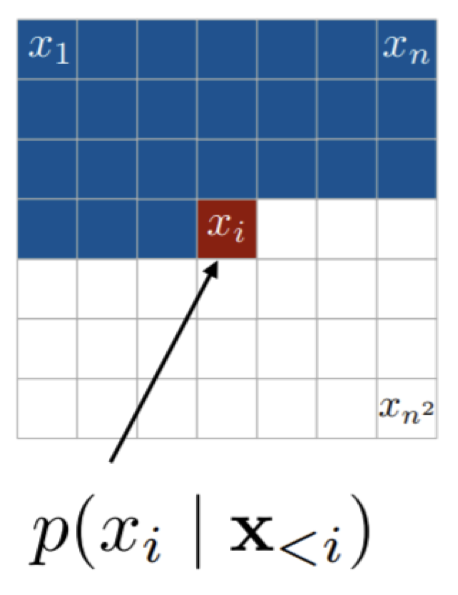
\includegraphics[width=0.3\columnwidth]{figures/pixelcnn.png}
%     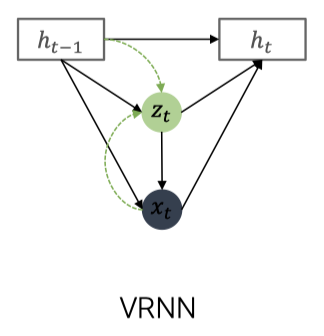
\includegraphics[width=0.4\columnwidth]{figures/VRNN.png}
% \end{center}

\subsection*{Temporal causal NN (TCN): WaveNet}

Idea: Adapt PixelCNN to Audio.

Prob: larger dim than images (\(>16000/{s}\)).

Trick: Dilated Conv, exponential increase in receptive field. (Stride Conv not allow to preserve resolution)

\subsection*{Variational RNN}

\textbf{Goal} increase expressiveness, noise robustness by stochastic latent variables into hidden state of an RNN.

\textbf{Model}
(1) Deterministic transition \(h_{t}=f_{\theta}(h_{t-1}, x_{t}, z_{t})\).
(2) Dynamic prior \(p_{\theta}(z_{t} | h_{t-1})\), overall prior \(p_{\theta}(z)=\prod_{t=1}^{T} p_{\theta}(z_{t}|z_{<t}, x_{<t}) = \prod_{t=1}^{T} p_{\theta}(z_{t} | h_{t-1})\times\) \( p_{f_\theta}(h_{t-1} | h_{t-2}, z_{t-1}, x_{t-1})\). Each $z_t$ depends on previous $x_{<t}$ and $z_{<t}$.

\textbf{Adv} for \(z\) in \(f_{\theta}\): (1) robust by randomness of \(z\) (2) latent \(z\) is high level, more informative on future.

\textbf{{Dec}}: \(p(x_{t} | z_{t})=g^{\text{out}}(h_{t-1}, z_{t})\),

\textbf{{Enc}}: \(q_{\phi}(z | x)=\prod_{t=1}^{T} q_{\phi}(z_{t} | x_{t}, x_{<t}, z_{<t})\),

\textbf{{ELBO}} \(\sum_t \log p_{\theta}(x_{t}|x_{< t}) \geq \mathcal{L}_{\theta, \phi}=\sum_{t=1}^{T} \mathbb{E}_{q_{\phi}(z_{t} | x_{t}, x_{<t}, z_{<t})}[\log p_{\theta}(x_{t} | z_{t}, z_{<t}, x_{<t})]-\KL(q_{\phi}(z_{t} | x_{t}, x_{<t}, z_{<t}) \| p_{\theta}(z_{t} | z_{<t}, x_{<t}))\).

KL in VRNN: (1) balance the informative \(z_t\) from \(x_t\) dependent \(q_\phi\) (if not \(x_t\) depend, \(z_t\) mostly from \(h_{t-1}\)) and overfit to memorize \(x_t\) by KL to prior. (2) Force the prior also to be informative from \(h_{t-1}\).


\subsection*{Conditional VRNN}

Hidden state \(\{z_t, \pi_t\}\).
Priors: \(p(z_{t} | h_{t-1})=g^{p, z}(h_{t-1})\), \( p(\pi_{t} | h_{t-1})=g^{p, \pi}(h_{t-1})\).
Transition: \(h_{t}=\tau(x_{t}, z_{t}, \pi_{t}, h_{t-1})\)
\textsf{{D}}: \(p(x_{t} | z_{t}, \pi_{t})=g^{\text {out}}(z_{t}, \pi_{t})\) (no \(h_{t-1}\) here).
\textsf{{E}}: \(q(z_{t} | x_{t})=g^{q, z}(h_{t-1}, x_{t}) \), \( q(\pi_{t} | x_{t})=g^{q, \pi}(h_{t-1}, x_{t})\).\\
\textsf{{ELBO}}: \( \sum_{t=1}^{T} \mathbb{E}_{q(z_{t}, \pi_{t}  x_{t})} \log p(x_{t}  z_{t}, \pi_{t})- \KL (q(z_{t}  x_{t}) \| p(z_{t})) - \KL(q(\pi_{t}  x_{t}) \| p(\pi_{t}))\)

\textbf{APP} Digital Handwriting Modeling.

\subsection*{Summary}
\textbf{Pros} \(p(x)\) tractable, explicit NLL metric to compare performance, easy to train, sample.
\textbf{Cons} Slow, no natural latent variable representation (except C-VRNN, STCN).
% \begin{center}
%     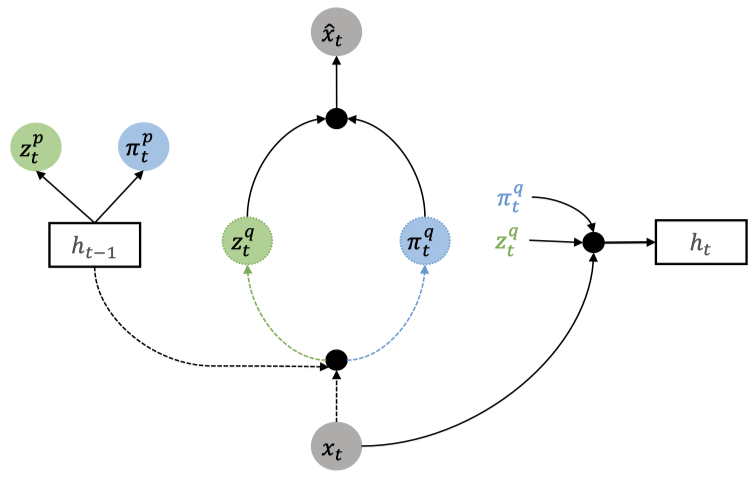
\includegraphics[width=0.7\columnwidth]{figures/C-VRNN.png}
% \end{center}

\subsection*{Self-attentioan and Transformers}

\(X=\operatorname{softmax}({({W}_{{Q}} {X})({W}_{{K}} {X})^{\top}}/{\sqrt{D}}+M) \odot {W}_{{V}} {X}\), mask \(M\) prevent accessing future. 

\textbf{Positional Encoding} unique sinusoidal encoding to preserve ordering. \(\mathsf{PE}_{i, t} =  \sin\text{/}\cos (\omega_{k} t)\) for \(i= 2k\text{/} 2k+1\), \(\omega_{k}=10000^{-{2 k}/{d}}\), \(t\) position in seq, \(i\) component in embedding vec.
Cost \(O(T^2 D)\).

\textbf{Trick} multi-head attention.

\textbf{APP} 3D human pose and mesh recon, 3D objects Mesh generation, 3D human motion modelling.

\subsection*{LLM / GPT}

Needs tokenization, can be finetuned by combining unsupervised pretraining $L_1(X) = \sum \log P(x_i|x_{i-1:i-k})$ plus supervised finetuning $L_2(X,Y) =$ $ \sum \log P(y|x\dots)$, then $L=L_2(X,Y) + \lambda L_1(X)$

For \textbf{autoreg. image/video generation}: problems with image quality, computational requirements. Solution: quantize images into tokens (e.g. Vector-Quantized \textbf{VQ-VAE} uses CNN enc/dec): lower dimensionality, more semantically meaningful. Also, can use LLMs.

% Application: 
% 3D human pose and mesh reconstruction: Conditioned on input image. Initializing 3D joints and 3D mesh vertex positions with T-pose. Refining 3D joints and 3D mesh vertices via self-attention. Randomly masking some joints and vertices to improve robustness., 


% Mesh generation for 3D objects: Given the current set of vertices V, estimates a predictive distribution for the next vertex coordinates z, y and x or a stopping token. \(p(\mathcal{V}^{{seq}} ; \theta)=\prod_{n=1}^{N_{V}} p(v_{n} | v_{<n} ; \theta)\), Similar to PixelCNN and WaveNet, 3D vertex coordinates are quantized and represented via discrete random var.

% The face model takes collection of vertices, as input a and the current sequence of face indices, and outputs a distribution over vertex indices. \(p(\mathcal{F}^{{seq}} | \mathcal{V} ; \theta)=\prod_{n=1}^{N_{F}} p(f_{n} | f_{<n}, \mathcal{V} ; \theta)\)


% 3D human motion modelling: Given a sequence of past frames, predicts the future. Decoupled attention over the temporal and spatial dimensions. To predict a joint in the next step, aggregates information from the past instances of the same joint and other joints at the current step.
\end{sectionbox}
\begin{sectionbox}{olive}\section{GANs, implicit model, neural sampler, likelihood-free model}

\textbf{Intuition} Likelihood not good indicator for generation, can be independent: \(\ln [0.01 p_{\text{true}}+0.99 q_{\text{noise}}] \geq \ln [0.01 p_{\text{true}}]=\ln p({x})-\ln 100\).

\textbf{Idea} Two-player game. \textbf{Generator} fool the discriminator with real-looking images \(G: \mathbb{R}^{Q} \to \mathbb{R}^{D}\) from Gaussian noise to images. \textbf{Discriminator} distinguish btw real and fake img \(D: \mathbb{R}^{D} \to [0,1]\) (0=fake\!)\!.

\textbf{Objective} \( \operatorname{argmin}_G \max_D {V}_{{G}, {D}}=\mathbb{E}_{x \sim p_d} [\ln D({x})] + \mathbb{E}_{\hat{x} \sim p_g} [\ln (1-D(\hat{{x}}))] = \mathbb{E}_{x \sim p_d} [\ln D({x})] + \mathbb{E}_{\hat{z} \sim p_z} [\ln (1-D(G(z)))]\)

\textbf{Optimal} \(D^{*} = \operatorname{argmax}_D {V}_{{G}, {D}} = \frac{p_{\text{D}}({x})}{p_{\text {D}}({x})+p_{\text {M}}({x})}\), proof by turning $\mathbb{E}$ into integrals and solving for $0=\nabla_D$integral body (and ensure concave, $\nabla\nabla_D > 0$). Then \(V_{G, D^{*}} =  -\ln 4+2 \JS (p_{d}({x}) \| p_{m}({x}))\), global optim if \(p_{d}({x})\equiv p_{m}({x})\).

If \(G,D\) enough capacity (strong assumpt), each step can reach \(D^*\),  update \(p_{m}\) directly instead of its param, then \(V(p_{\text{M}}, D^{*})\) is convex, global optim can reach and \( \propto \sup _{D} \mathbb{E}_{p_{m}({x})} \ln (1-D({x})) d {x}\).

(1) In practice finding optimal \(D\) in inner-loop is computationally prohibitive and lead to overfitting on finite datasets.

(2) \textbf{Aim} keep \(D\) near optimum and \(G\) changes only slowly: \(k\) steps of optim \(D\) (typically \(k \in\{1, \ldots, 5\}\)), 1 step of optim \(G\) with small lr. 

(3) \(\log (1-D(G(z)))\) near zero \(\to\) smaller \(\nabla\) \(\Rightarrow\) gradient ascent \(\max _{G} \mathbb{E}_{z \sim p_{z}(z)}[\ln (D(G(z)))]\).

% Theoretical analysis shows that this minimax game recovers = \(p_{\text {M}}=p_{d a t a}\) if \(G\) and \(D\) are given enough capacity and  assuming that \(D^*\) can be reached. 

\subsection*{Issues}

1. Difficult to train, Mode collapse (no sample diversity), saddle point in dual energy landscape. Sol: unrolled GAN (simulate $k'$ more steps of $D$ to calculate grads for $G$, then revert to prev $D$).

2. Low dim manifolds in high dim prob space have little overlap. \(D\) of vanilla GAN saturates if no overlapping support. \(\JS\) only measures similarity, not `work' required from \(p_{\text {M}}\) to  \(p_{\text {D}}\). Sol: Wasserstein GAN. GAN can be generalized to entire family of div.

\subsection*{Pros and Cons}
\textbf{Pros} (1) A wide variety of functions and distributions can be modeled (flexibility). (2) Only backprop when training, no sampling, stochastic optim. (3)  No approximation to likelihood required as in VAEs. (4) Samples more realistic than other DGMs.

\textbf{Cons} (1) No explicit \(p_{M}\). (2) no direct means to evaluate likelihood (3) Careful balancing \(G\) and \(D\) during training. (4) lack of theory and learning algo wrt explicit models.

\subsection*{Applications}

\textbf{Progressive Growing of GAN}s:  Grow the generator and discriminator resolution by adding layers during training.

\textbf{StyleGAN} uses layer-wise style conditioning with AdaIN (see tutorial), allows style mixing at different layers.

\textbf{Pix2Pix} cond GAN, Obj: \(\mathcal{L}(G, D)=\mathcal{L}_{c G A N}(G, D)+\lambda \mathcal{L}_{L 1}(G)\), \(\mathcal{L}_{{cGAN}}(G, D)=\mathbb{E}_{x, y}[\ln D(x, y)]+\mathbb{E}_{x, z}[1-\ln D(x, G(x, z))]\), \(x\) conditions, \(\mathcal{L}_{L 1}(G)=\mathbb{E}_{x, y, z}[\|y-G(x, z)\|_{1}]\) reconstruction loss. Requires paired images as training data. Translates samples from two sides e.g. facade rectangles to facade img.

\textbf{CycleGAN} unpaired image translation: Two conditional GANs \(\mathcal{L}(G, F, D_{X}, D_{Y})=\mathcal{L}_{G A N}(G, D_{Y}, X, Y)+\mathcal{L}_{G A N}(F, D_{X}, Y, X)+\lambda \mathcal{L}_{\text {cyc }}(G, F)\), \(L_{cyc} = .=\mathbb{E}_{x \sim p_{\text {D}}(x)}\|\| F(G(x))-x \|_{1}]+\mathbb{E}_{y \sim p_{\text {D}}(y)}[\|G(F(y))-y\|_{1}]\). Transfer and Transfer back.

\textbf{BicycleGAN} both image and style cycle consistency.

\textbf{Vid2vid} uses $p(\tilde{y}_{1:T} \mid x_{1:T}) = \prod_{t=1}^{T} p(\tilde{y}_t \mid \tilde{y}_{t-L:t-1}, \, x_{t-L:t})$ to also use past frame.

% \textbf{GauGAN} Given semantic seg and reference style, synthesize image. Problem with pix2pix: Unconditional norm layer in \(G\) “washes away” information of semantic labels. Sol: Spatial cond norm \(\gamma_{c, y, x}^{i}({m}) \frac{h_{n, c, y, x}^{i}-\mu_{c}^{i}}{\sigma_{c}^{i}}+\beta_{c, y, x}^{i}({m})\)

\textbf{RLHF} used for training LLMs.

\textbf{3D Applications}: 3D-GAN outputs objects, PlatonicGAN uses 3D-GAN but converts back to 2D for training to make use of images, HoloGAN like PlatonicGAN but outputs 3D features that can be rendered with neural rendereing, EG3D uses tri-plane projections 3D representation and neural rendering

\end{sectionbox}
\begin{sectionbox}{cyan}\section{Normalizing Flows}
% Goal: a latent variable model with tractable likelihoods.
\textbf{Idea} \( p_{X;\theta}(x)=p_{Z}(f_{\theta}^{-1}(x))|\text{det}\partial_{x} f_{\theta}^{-1}(x)|\).
\textbf{Require} (1) NN differentiable, invertible, preserve the dim, (2) Jacobian computed efficiently.
\textbf{Trick} triangular matrix to reduce the complexity of Det to \(O(d)\).

Flow Trans:\({x} = f_{k} \circ f_{k-1} \circ \cdots f_{2} \circ f_{1}(z)\), \(p_{x}(x)=p_{z}(f^{-1}(x)) \prod_{k}|\text{det}\partial_{x} f_{k}^{-1}(x)| \)

% \textbf{ML} \(\log p_{x}({\mathcal{D}})=\sum_{x \in \mathcal{D}}\ln p_{z}(f^{-1}({x}))+\sum_{k} \ln|\text{det}\partial_{x} f_{k}^{-1}(x)| \).
% \textbf{Planner}: \(f(z)={z}+{u h}({w}^{T} {z}+{b})\), \(|\operatorname{det} \partial_{{z}} f |=|1+h^{\prime} {u}^{T} {w}|\).
% \textbf{Radial}: \(f({z})={z}+\beta h(\alpha, r)({z}-{z}_{0})\), \(r=|{z}-{z}_{0}|\), \(h(\alpha, r)=(\alpha+r)^{-1}\), \(|\operatorname{det} \partial_{{z}} f| = [1+\beta h(\alpha, r)]^{d-1}[1+\beta h(\alpha, r)+\beta h^{\prime}(\alpha, r) r]\)

\subsection*{Coupling Layer}
\textsf{$f$\!:\!}
\(\left(\begin{array}{c}
        y^{A} \\
        y^{B}
    \end{array}\right)=\left(\begin{array}{c}
        h(x^{A}, \beta(x^{B})) \\
        x^{B}
    \end{array}\right),\)
\textsf{$f^{-1}$\!:\!} \(\left(\begin{array}{l}
        x^{A} \\
        x^{B}
    \end{array}\right)=\left(\begin{array}{c}
        h^{-1}(y^{A}, \beta(y^{B}))) \\
        y^{B}
    \end{array}\right),\)
Jacob: \(\left(\begin{array}{cc}
        h^{\prime} & h^{\prime} \beta^{\prime} \\
        0          & 1
    \end{array}\right).\)\\
\(h(x) = (h(x_{1}), \ldots, h(x_{n}))^{\top}\) element-wise. \( \partial_{x^{\top}} h=\operatorname{diag}(h^{\prime}(x_{1}), \ldots, h^{\prime}(x_{n}))\).

Continuous NF: model infinite number of trans with proper temporal discretization. I.e. model the evolution of a neural ODE.

% \begin{center}
%     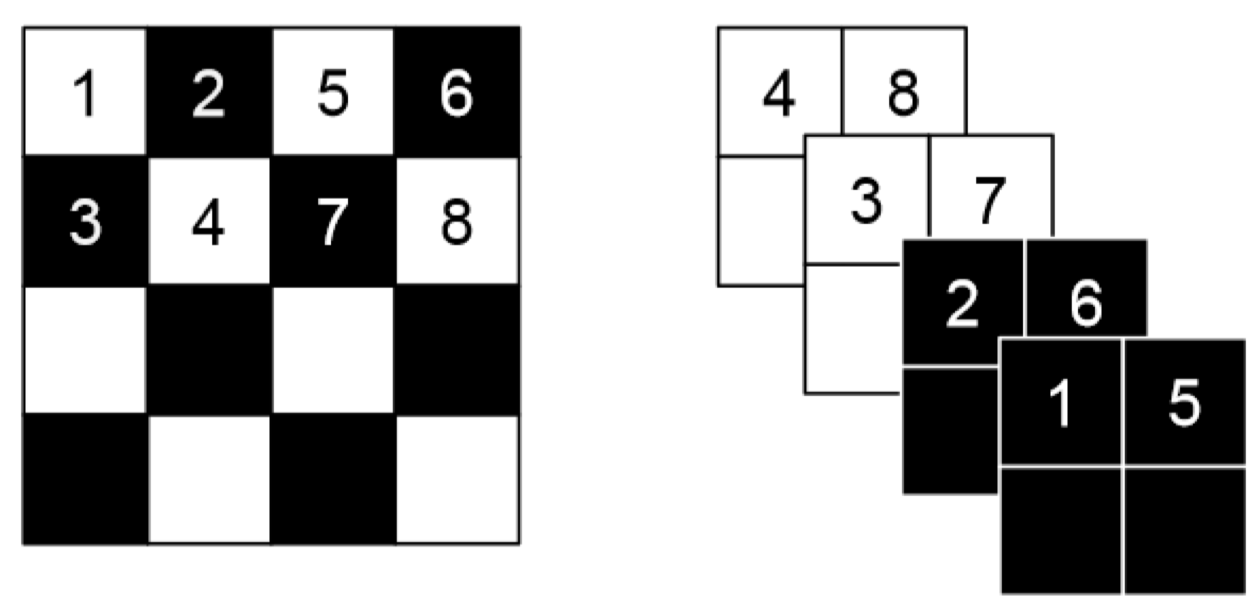
\includegraphics[width=0.8\columnwidth]{figures/coupling_layer.png}
% \end{center}

\subsection*{Multiscale architecture, \textit{FB = step of flow}}

x -> [Squeeze, [FB1, FB2, FB3]$\cross K$,  Split -> $z_i$]$\cross (L-1)$, Squeeze, [FB1, FB2, FB3]$\cross K$ -> $z_L$

Squeeze reduces spatial dimensions (and increases num of channels). Split outputs half of the features $z$ (so it iteratively gets smaller).

\subsection*{FB1 - activation norm}
Scale and bias per channel, sim to BN, data depend, trainable.
\textsf{F} \( y_{i, j}={s} \odot x_{i, j}+{b}\),
\textsf{R} \( {x}_{i, j}=({y}_{i, j}-{b}) / {s}\),
\textsf{LogDet} \(\mathrm{H} \cdot W \cdot \operatorname{sum}(\log |s|)\).

\subsection*{FB2 - invertible 1x1 conv}

\textsf{F} \({y}_{i, j}={W} {x}_{i, j}\)
\textsf{R} \({x}_{i, j}={W}^{-1} {y}_{i, j}\)
\textsf{LogDet} \(h \cdot w \cdot \log |\operatorname{det}{W}|\), \({W}:[c \times c]\),
\(O(c^3)\) for \(|\operatorname{det}{W}|\)  reduce to \(O(c)\) by \({W}={P L}({U}+\operatorname{diag}({s}))\), \(\log |\operatorname{det}{W}|=\operatorname{sum}(\log |{s}|)\).


\subsection*{Fb3 - (conditional) affine coupling layer}

\textbf{Conditional operation} \(\beta(x^{B};C)\).

% \begin{center}
%     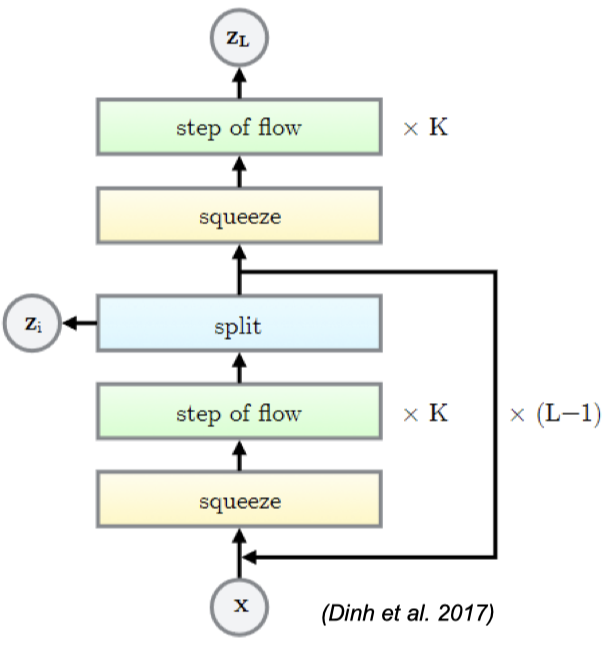
\includegraphics[width=0.5\columnwidth]{figures/flow_block.png}
% \end{center}

\subsection*{Application}

\textbf{Super-Res Flow} learns a distribution of HR variants. Cond on a low-res image.  Pretrained CNN encodes a low-resolution image: \({u}=g_{\theta}({x})\) inject to actnorm, affects all channels and spatial locations. \textsf{F} \({h}^{n+1}=\exp (f_{{\theta}, s}^{n}({u})) \cdot {h}^{n}+f_{{\theta}, b}({u})\), \textsf{R} \({h}^{n}=\exp (-f^{n} {\theta}, s({u})) \cdot({h}^{n+1}-f^{n} {\theta}, b({u}))\), \textsf{LogDet} \(\sum_{i j k} f^{n} {\theta}_{, s}({u})_{i j k}\).


\textbf{StyleFlow}(cmp to StyleGAN) Replace mapping network with a continuous normalizing flow, Condition on image attributes.


\textbf{C-Flow} with two flows

Conditioning \(Flow_A\): Standard affine coupling layer, to images.

Conditioned \(Flow_B\): trans param conditioned on, to point cloud, sketch, seg, etc.

\textbf{Applications} (1) (multimodal) image-to-image mapping (2) style transfer (3) image manipulation (4) 3D point cloud reconstruction from images. (5) Probabilistic Modeling for Human Mesh Recovery (6) PointFlow: 3D Point Cloud Generation (7) but long training and low res

\subsection*{Difficulty for generative model}
Evaluating \(\log p(x)\) is hard and usually computationally not tractable.
\end{sectionbox}
\begin{sectionbox}{orange}\section{Diffusion \& Foundation models}
\end{sectionbox}
\begin{sectionbox}{purple}\section{Parametric Body Models}
\textbf{Challenge} rotation, foreshortening, scaling, intra-category variation, aspect ratio.

\subsection*{2D Body Modeling \textnormal{\textit{(all fully supervised)}}}

\textbf{Pictorial Structures} body made of cylinders and springs, minimize how well image matches + how much body deforms: \( \argmin_L \sum_{i=1}^{n}m_i(l_i) + \sum_{(v_i,v_j)\in E} d_{ij}(l_i,l_j) \)

\textbf{Direct Regression} ConvNet output \((x,y)\) for certain body parts; \textbf{Iterative Error Feedback} refines on smaller sorrounding area; better with Gaussian heatmap.

\textbf{Convolutional Pose Machines} iteratively predicts whole heatmap w/ increasing receptive field; \textbf{OpenPose} adds Part Affinity Fields / associativity vectors \textit{btmup}; \textbf{ViTPose} transformer encoder-decoder \textit{tpdwn}.

\subsection*{3D face: Statistical Shape Models}

Obtain vertex correspondences (i.e. registration) w/ bootstrapping; shapes $S_i$ in full correspondence, $\bar{S}$ avg, $x_i=S_i-\bar{S}$ in mat $X$, covariance $C=\frac{1}{m}X X^\intercal=\frac{1}{m}U \text{diag}(\sigma_i^2)U^\intercal$ (SVD), $c_i = U^\intercal x_i$, full model \( S = \bar{S} + \sum_{i=1}^{m} c_i \sigma_i u_i\).

\subsection*{3D: SMPL Skinned Multi-Person Linear}

\(S=M(\makebox[0pt][l]{\smash{\text{\raisebox{0.75em}{\tiny{pose shape}}}}}\theta, \;\beta)
=W(T_P(\beta, \theta), J(\beta), \theta, \mathcal{W})\)

\(T_P(\beta, \!\theta) \!\!=\!\! \bar{T} \!\!+\!\! B_S(\beta) \!\!+\!\! B_P(\theta)\); \(J(\beta) \!\!=\!\! \mathcal{J}\!\!\cdot\!(\bar{T} \!\!+\!\! B_S(\beta))\)

\(B_S(\beta,\!\mathcal{S})=\sum_{i=1}^{|\beta|} \beta_n S_n\) \;\;\;\; $\text{\raisebox{-0.3em}{$\downarrow$}} R$ {\tiny flat rotation matrices}

\(B_P(\theta,\mathcal{P})=\sum_{i=1}^{9K}(R(\theta)-R(\theta^*))_n P_n\)

\(V'=\{t_i\}_{i=0}^N = R_0(T_P(\beta,\theta)-j_0) + j_0 + t\)

{\color{black!60} \tikz[baseline=(math.base)] \node[opacity=0.6, inner sep=0pt] (math) {\(t'_i = \sum_{k=1}^{K}w_{k,i} G'_k(\theta, J) t_i\)}; \;\; plain LBS}

\(t'_i = \sum_{k=1}^{K}w_{k,i} G'_k(\theta, J(\beta)) (t_i \!\!+\!\! b_{S,i}(\beta) \!\!+\!\! b_{P,i}(\theta))\)

\vspace{3pt}
$W$ Linear Blend Skipping fun, factored model (shape and pose separate); $\mathcal{W} \in \mathbb{R}^{K' \text{\tiny{$\!\!\!\!\leq\!\!\! 4$}} \text{\raisebox{0.2em}{$\cross$}} 3N \text{\tiny{$\!\!=\!\! 6890$}}}$ skinning weights; $\beta$ 10 shape params; $\theta \in \mathbb{R}^{3K+3}$ joint angles for $K\text{\tiny{$\!\!=\!\!23$}}$ joints in angle-axis form wrt to parent; $\bar{T}\in\mathbb{R}^{3N}$ rest pose; $B_S, B_P \in\mathbb{R}^{3N}$ shape/pose blend shapes;  $J: \mathbb{R}^{|\beta|} \rightarrow \mathbb{R}^{3K}$ joint mapper; $\mathcal{J}$ regression matrix learned w/ least squares; $\mathcal{S}$ shape displacements learned w/ PCA; $\mathcal{P}$ blend shapes / pose correctives learned; $R_0, t$ global root orientation/translation (\textit{not} wrt root!), $j_0$ root joint, $V'$ template vertices; $G'_k$ \vspace{-2.5pt} global transform; $\Phi = \{\bar{T}, \mathcal{W}, \mathcal{J}, \mathcal{S}, \mathcal{P}\}$.

\vspace{3pt}
\textbf{Registration} chicken-and-egg, so solve model and registration jointly. First \textbf{train} $\{\mathcal{W}, \mathcal{J}, \mathcal{P}\}$ by minimizing surface reconstr. error on multi-pose dataset; regularize $\mathcal{P}$ to 0, $\mathcal{W}$ to good initial, $\mathcal{J}$ to be local. Then
\vspace{-2.3pt} train $\{\bar{T}, \mathcal{S}\}$ w/ PCA using multi-shape normalized pose dataset (so no pose contribs in shape space), separate models for men and women.

(1) Pose Parameter Training, linear comb of following loss:
1. \(E_D\): \(L_2\) loss btw registerd and model vertices.
2. \(E_Y\): symmetry regularization on vertice and joints.
3. \(E_J\): \(J(\vec{\beta} ; \mathcal{J}, \overline{\mathbf{T}}, \mathcal{S})\) close to default \(J\).
4. \(E_{P}(\mathcal{P})=\|\mathcal{P}\|_{F}^{2}\) prevent overfitting of pose-dependent blend shape.
5. \(E_{W}(\mathcal{W})=\|\mathcal{W}-\mathcal{W}_{I}\|_{F}^{2}\) blend weights towards initial weights

Non-negative least squares with additional term that encourages the weights to add to one works best for \(\mathcal{J}\).

(2) Shape Parameter Training: 1. estimate pose \(\theta\) from generic shape \({\arg \min}_{{\vec{\theta}}} \sum_{e}\|W_{e}(\hat{\mathbf{T}}_{\mu}^{P}+B_{P}(\vec{\theta} ; \mathcal{P}), \hat{\mathbf{J}}_{\mu}^{P}, \vec{\theta}, \mathcal{W})-\mathbf{V}_{j, e}^{S}\|^{2}\),
2. get shape-dep. vertices \(\hat{\mathbf{T}}_{j}^{S}={\arg \min }_{\hat{\mathbf{T}}} \|W(\hat{\mathbf{T}}+B_{P}(\vec{\theta}_{j} ; \mathcal{P}), \mathcal{J} \hat{\mathbf{T}}, \vec{\theta}_{j}, \mathcal{W})-\mathbf{V}_{j}^{S}\|^{2}\).
3. PCA on \(\{\hat{\mathbf{T}}_{j}^{S}\}_{j=1}^{S_{\text {subj }}}\) to obtain \(\{\overline{\mathbf{T}}, \mathcal{S}\}\)

\textbf{DMPL: Dynamic SMPL} Additional term for velocity and acceloration. \textbf{Clothing} can be represented with offsets from SMPL (hard to train), or with implicit surfaces (performance heavy).

\textbf{Human Mesh Recovery (HMR)}: regresses $\theta, \beta$ and camera from 2D. Uses 2D reprojection loss and discriminator loss to tell if similar to priors.

\textbf{Optimization Based Fitting} / \textbf{SMPLify}: like HMR but uses 2D keypoint objective for reprojection loss. \(\Theta^{t+1} = \Theta^t - \lambda\left(\derivative{L_{reproj}}{\Theta} + \derivative{L_{prior}}{\Theta}\right)\). But hand-crafted, slow to converge, sensitive to initialization.

\textbf{Learned Gradient Descent (LGD)}

\(\Theta^{t+1}=\Theta^{t}+F(\derivative{L_{\text {reproj}}}{\Theta}, \Theta^{t}, x)\), \(F\) is NN.

\textbf{Learned iterative fitting} (when IMU/EM sensors instead of img) iteratively fit model with RNN, reproject by simulating sensor measurements, minimize with LGD.

% \textbf{Spring Models, Pictorial Structure Model}
% %
% minimize deg of mismatch \(S(I, L)=\sum_{i \in V} \alpha_{i} \cdot \phi(I, l_{i})+\sum_{i j \in E} \beta_{i j} \cdot \psi(l_{i}, l_{j})\), \(\phi\) unary term, likelihood this patch of image for this part \(i\), \(\psi\) pairwise term btw part \((i,j)\) with spring model \(\beta\).

% \textbf{PSM with Flexible Mixtures} \(S(I, L, M)=\sum_{i \in V} \alpha_{i}^{m_{i}} \phi(I, l_{i})+\sum_{i j \in E} \beta_{i j}^{m_{i} m_{j}} \psi(l_{i}, l_{j})+S(M)\), \(m_i\) stands for mixture type \(m_i\), e.g. orientation. \(S(M)=\sum_{i j \in E} b_{i j}^{m_{i} m_{j}}\) co-occurrence bias, prior knowledge about mixture part co-occurrence likelihood.

% \subsection*{Feature Representation Learning}
% \textbf{Direct Regress} ConvNet output \((x,y)\) for certain body parts.

% \textbf{Heatmaps} ConvNet, each keypoint with separate binary heatmap. Keypoint positive, else negative. usually Gaussian blured around keypoint.

% \textbf{Conv Pose Machine} iteratively generate heatmaps, then with original img generate more accurate heatmap.

% \textbf{Think-slicing Networks} combine conv feature + body struct. Energy term for a seq of slice/frame + temporal displace for each part \(S_{\text {slice}} = \sum_{t=1}^{T} S(I^{t}, p^{t})+\sum_{(i, i^{*}) \in E_{f}} \psi_{i, i^{*}}(p_{i}, p_{i^{*}}^{\prime})\), \(\psi_{i, j}(p_{i}, p_{j})=w_{i, j} \cdot d(p_{i}-p_{j})\). \( d(p_{i}-p_{j})=[\Delta x, \Delta x^{2}, \Delta y, \Delta y^{2}]^{\top}\).

% \textbf{Inference} \(\operatorname{score}_{i}(p_{i}) = \phi_{i}(p_{i} | I)+\sum_{k \in \text{child}(i)} m_{k i}(p_{i})\), \(m_{k i}(p_{i}) = \max _{p_{k}}(\operatorname{score}_{k}(p_{k})+\psi_{k, i}(p_{k}, p_{i}))\) in a bottom up manner. Use subgradient for \(\max\) operator when training.

% \subsection*{3D human Pose and Shape: SMLP}
% % Usage for 3D: (1) infer peoples intention in sensitive places like stations, predict pedestrains motion in the self driving car (3) robots could help olderies once understand the action (4) recon skeleton in 3D for VR/AR gaming (5) analyze sports match
% \textbf{Representation} 3D mesh (\~ 7000 vertices and faces). Design mesh (by artist) to align unordered scans and incomplete 3D points from raw scan.

% \textbf{Challenge} Chicken-and-egg problem, solve model and registration jointly.

% \textbf{Linear Blend Skinning (Naive)} \(\mathbf{t}_{i}^{\prime}=\sum_{k} w_{k i} \mathbf{G}_{k}(\boldsymbol{\theta}, \mathbf{J}) \mathbf{t}_{i}\)  \(\mathbf{t}, \mathbf{t}^{\prime}\) rest/trans vertices, \(w_{ki}\) blend skinning weights, \(G_k\) rigid bone transformation, \(\theta\) pose, \(J\) Joint locations.

% \textbf{Result} creates artifact, cuz unified blending weights try to cover all kinds of trans.

% \textbf{SPML-LBS}
% \textbf{idea}  pose/shape dependent rest pose.

% \(T_{P}(\vec{\beta}, \vec{\theta})=\overline{\mathbf{T}}+B_{S}(\vec{\beta})+B_{P}(\vec{\theta})\), \(\beta\) body shape param,
% \textit{shape blend shape} \(B_{S}(\vec{\beta} ; \mathcal{S})=\sum_{n=1}^{|\vec{\beta}|} \beta_{n} \mathbf{S}_{n}\),
% \textit{pose blend shape} \(B_{P}(\vec{\theta} ; \mathcal{P})=\sum_{n=1}^{9 K}(R_{n}(\vec{\theta})-R_{n}(\vec{\theta}^{*})) \mathbf{P}_{n}\), \(\theta^*\) rest pose.

% Joint location dependency \(J(\vec{\beta} ; \mathcal{J}, \overline{\mathbf{T}}, \mathcal{S})=\mathcal{J}\times(\overline{\mathbf{T}}+B_{S}(\vec{\beta} ; \mathcal{S}))\),
% \(\mathcal{J}\) regression matrix from rest verticese to rest joints,

% Overall Mesh \(M(\vec{\beta}, \vec{\theta} ; \Phi)\): \(\overline{\mathbf{t}}_{i}^{\prime}=\sum_{k=1}^{K} w_{k, i} G_{k}^{\prime}(\vec{\theta}, J(\vec{\beta}))(\overline{\mathbf{t}}_{i}+\mathbf{b}_{S, i}(\vec{\beta})+\mathbf{b}_{P, i}(\vec{\theta}))\).

% \textbf{Model param} \(\Phi=\{\overline{\mathbf{T}}, \mathcal{W}, \mathcal{S}, \mathcal{J}, \mathcal{P}\}\).

% \textbf{Train} First \(\{\mathcal{J}, \mathcal{N}, \mathcal{P}\}\) with multi-pose dataset, then \(\{\overline{\mathbf{T}}, \mathcal{S}\}\) with multi-shape dataset, separate models for men and women.

% (1) Pose Parameter Training, linear comb of forllowing loss:

% 1. \(E_D\): \(L_2\) loss btw registerd and model vertices.
% 2. \(E_Y\): symmetry regularization on vertice and joints.
% 3. \(E_J\): \(J(\vec{\beta} ; \mathcal{J}, \overline{\mathbf{T}}, \mathcal{S})\) close to default \(J\).
% 4. \(E_{P}(\mathcal{P})=\|\mathcal{P}\|_{F}^{2}\) prevent overfitting of pose-dependent blend shape.
% 5. \(E_{W}(\mathcal{W})=\|\mathcal{W}-\mathcal{W}_{I}\|_{F}^{2}\) blend weights towards initial weights

% Non-negative least squares with additional term that encourages the weights to add to one works best for \(\mathcal{J}\).

% (2) Shape Parameter Training:

% 1. estimate pose \(\theta\) from generic shape \({\arg \min}_{{\vec{\theta}}} \sum_{e}\|W_{e}(\hat{\mathbf{T}}_{\mu}^{P}+B_{P}(\vec{\theta} ; \mathcal{P}), \hat{\mathbf{J}}_{\mu}^{P}, \vec{\theta}, \mathcal{W})-\mathbf{V}_{j, e}^{S}\|^{2}\),
% 2. get shape-depend vertices \(\hat{\mathbf{T}}_{j}^{S}={\arg \min }_{\hat{\mathbf{T}}} \|W(\hat{\mathbf{T}}+B_{P}(\vec{\theta}_{j} ; \mathcal{P}), \mathcal{J} \hat{\mathbf{T}}, \vec{\theta}_{j}, \mathcal{W})-\mathbf{V}_{j}^{S}\|^{2}\).
% 3. PCA on \(\{\hat{\mathbf{T}}_{j}^{S}\}_{j=1}^{S_{\text {subj }}}\) to obtain \(\{\overline{\mathbf{T}}, \mathcal{S}\}\)


% \textbf{DMPL: Dynamic SMPL} Additional term for velocity and acceloration.


% \subsection*{SMPL Estimation Methods}

% \textbf{Optimization Based Fitting} SMPLify: (1) Given image, pass to DNN to get \(\beta, \theta\), (2) from SMPL get joints, (3) \(\theta^{*}={\operatorname{argmin}}_{\theta} \| \text{Joint diff}\| + \text{Prior Reg}\)

% Cons: (1) Hand-crafted optimization routine. (2) Sensitive to initialization (3) Slow convergence.

% \textbf{Learned Gradient Descent (LGD)} \(\theta^{t+1}=\theta^{t}+F(\partial_{\theta} L_{\text {reproj}}, \theta^{t}, x)\), \(F\) is NN.

% Train: render with different views current pose \(\to\) learn how to optimize.

% \textbf{APP}:Football match pose estimation

% \subsection*{From key points to detailed 3D surface}

% Challenges: Self-occlusion, lack of depth info, articulated motion,  mon-rigid deformation (clothing)

% \textbf{Templated-based Capture}

% (1) capture body with template cloth model  (2) rack cloth model deformation with time. Cons: Laborious preprocessing, No public access to models \(\to\) Automatic and general pipeline required.

% \textbf{Regression-based Reconstruction} recover every pixel.

% \textbf{Templated-based + Regression-based}
\end{sectionbox}
\begin{sectionbox}{green}\section{Implicit Surfaces and Neural Radiance Fields}
3D representations: Voxels (Discretization of 3D space into grid), Points cloud, meshes (vertices and faces).

\subsection*{Implicit shape representation}
Represent surface as the zero level-set of a continuous function \(S = \{x: f(x) = 0\}\).

\subsection*{Neural IR (NIR)}

\textbf{Occupancy Networks} \(f_{\theta}: \mathbb{R}^{3} \times \mathcal{X} \rightarrow[0,1]\), 3D location and  condition as input, output probability

\textbf{signed distance field: DeepSDF} \(f_{\theta}: \mathbb{R}^{3} \times \mathcal{X} \rightarrow \mathbb{R}\), output shape represented by \(f\theta(p) = \tau\).

\textsf{Supervise NIR from Other representation}:

(1) \textbf{Watertight meshes} Query GT occupancy or SDF from GT meshes, Train with cross-entropy loss.

(2) \textbf{Points cloud: Implicit Geometric Regularization (IGR)} unordered and hard, \(\chi=\left\{x_{i}\right\}_{i \in I} \subset \mathbb{R}^{3}\)), learn \(f_{\theta}(x)\) is approximately the signed distance function to a plausible surface \(M\) defined by \(\chi\).
% 
Continuous Shortest Path (Eikonal PDE), \(\|\nabla f(x)\|= v^{-1}(x)\) for \(x \in \Omega_{0} \subset \mathbb{R}^{n}\), \(f(x)=q(x) \text { for } x \in \Omega_{T}\). When \(v(x) = 1\), learned function \(f\) is approximately the distance to the suface.
% 
Loss: \(\mathcal{L}(\theta)=\sum_{i \in I}\left|f_{\theta}\left(x_{i}\right)\right|^{2}+\lambda \mathbb{E}_{x}\left(\left\|\nabla_{x} f_{\theta}(x)\right\|-1\right)^{2}\).
% 
Many solutions, local minima. SGD for NN is used as implicit regularization.

(3) \textbf{Images: Differentiable Volumetric Rendering (DVR)}
% 
NN output texture/color \(t_\theta(p)\) and occupancy \(f_\theta(p) \in [0, 1]\).
% 
\textbf{Forward}
1. given observation position \(\mathbf{r}_0\) and relative pixel \(\to\) direction of the ray \(\mathbf{w}\),
2. find the solution \(d\) for surface, \(f_\theta (\mathbf{p} = \mathbf{r}_0 + d \mathbf{w}) = \tau\),
3. use \(t_\theta(\mathbf{p} = \mathbf{r}_0 + d \mathbf{w})\) for texture and color. Secant method for linesearch of zero point \(x_{2}=x_{1}-f\left(x_{1}\right) \frac{x_{1}-x_{0}}{f\left(x_{1}\right)-f\left(x_{0}\right)}\)

\textbf{Backward}
1. Loss: differnce w.r.t images, \(\mathcal{L}(\hat{\mathbf{I}}, \mathbf{I})=\sum_{\mathbf{u}}\left\|\hat{\mathbf{I}}_{\mathbf{u}}-\mathbf{I}_{\mathbf{u}}\right\|\),
% 
\(\frac{\partial \mathcal{L}}{\partial \theta}=\sum_{\mathbf{u}} \frac{\partial \mathcal{L}}{\partial \hat{\mathbf{I}}_{\mathbf{u}}} \cdot \frac{\partial \hat{\mathbf{I}}_{\mathbf{u}}}{\partial \theta},
% 
\frac{\partial \hat{\mathbf{I}}_{\mathbf{u}}}{\partial \theta}=\frac{\partial \mathrm{t}_{\theta}(\widehat{\mathbf{p}})}{\partial \theta}+\frac{\partial \mathrm{t}_{\theta}(\widehat{\mathbf{p}})}{\partial \widehat{\mathbf{p}}} \cdot \frac{\partial \widehat{\mathbf{p}}}{\partial \theta}\),
2. From \(f_{\theta}(\widehat{\mathbf{p}})=\tau\) and \(\widehat{\mathbf{p}}=\mathbf{r}_{0}+\hat{d}(\theta) \mathbf{w}\) \(\to\) implicit gradient \(\frac{\partial \widehat{\mathbf{p}}}{\partial \theta}=-\mathbf{w}\left(\frac{\partial f_{\theta}(\widehat{\mathbf{p}})}{\partial \widehat{\mathbf{p}}} \cdot \mathbf{w}\right)^{-1} \frac{\partial f_{\theta}(\widehat{\mathbf{p}})}{\partial \theta}\).


\subsection*{Neural Radiance Field (NeRF)}
\textbf{Motivation} Surfaces are good, but scenes are more complex.

\textbf{Network} \(F_\theta(x,y, z, \theta, \phi) = (r,g,b, \sigma)\), \(\sigma\) output density.

\((\theta, \phi)\) view direction, added at late stage of network, cuz most of the texture is not view dependent, othervise, will fall into trivial solution of sphere with complex texture. Density (geometry) is independent of viewing direction. Viewing direction only applied at a later layer, which limits the viewdependent effects and thus encourages detailed geometry.

\textbf{Volume Rendering}
% 
\(\alpha=1-\mathrm{e}^{\left(-\sigma_{i} \delta_{i}\right)}, \delta_{i}=t_{i+1}-t_{i}\), Transmittance \(T_{i}=\prod_{j=1}^{i-1}\left(1-\alpha_{j}\right)\), color \(c=\sum_{i=1}^{N} {T_{i} \alpha_{i}} c_{i}\).

\textbf{Train} \(\min _{\theta} \sum_{i}\left\|\operatorname{render}_{i}\left(F_{\theta}\right)-I_{i}\right\|^{2}\), sampling efficiency is a big issue.

\textbf{trick: Positional encoding} pass low-dim \(x,y,z\) coordinates via fixed positional encoding controlled by \(L\) or random Fourier features of varying frequencies, instead of directly use \((x,y,z)\). 
% 
\(\mathsf{PE} = \text{cat}[\cos k\mathbf{v}, \sin k\mathbf{v}]_{k=1}^{2^L}\), 
% 
or \(\gamma(\mathbf{v})=[\cos (\mathbf{B v}), \sin (\mathbf{B v})] \quad \mathbf{B} \sim \mathcal{N}\left(0, \sigma^{2}\right)\), too big mapping bandwith  \(\sigma\) leads to noisy images (overfit).
\end{sectionbox}
\begin{sectionbox}{brown}\section{Tutorials}

\textbf{Loss} Mean Sq Err: $L_{\text{MSE}} $ $= \frac{1}{n} \sum_{i=1}^{n} (y_i - \hat{y}_i)^2$; Binary Cross Entropy $L_{\text{BCE}} = -\frac{1}{n} \sum_{i=1}^{n} \left[ y_i \log(\hat{y}_i) + (1 - y_i) \log(1 - \hat{y}_i) \right]$; Categorical Cross Entropy $L_{\text{CCE}} = -\sum_{i=1}^{n} \sum_{j=1}^{C} y_{ij} \log(\hat{y}_{ij})$; Hinge loss $L_{\text{Hinge}} = \frac{1}{n} \sum_{i=1}^{n} \max(0, 1 - y_i \hat{y}_i)$.

\textbf{Regularization} (+ loss) L1 $||\theta||_1$,  L2 $\tfrac{1}{2}||\theta||_2^2$

\textbf{Dropout} at training time disable node $j$ in layer $l$ w/ prob $p$: $r_j^{[l]} \sim \text{Bernoulli}(p)$, then $\tilde{y}^{[l]}=r^{[l]} \odot y^{[l]}$; at inference time do weight scaling $\tilde{\theta} = \theta p$.

\textbf{Normalization} $\mu = \tfrac{1}{n} \sum x_i$; $\sigma^2 = \tfrac{1}{n-1} \sum (x_i - \mu)^2$, $x_{i}^N = (x_i-\mu) / \sqrt{\sigma^2}$.

\textbf{Batch norm.} $x_{i}^N = (x_i-\mu) / \sqrt{\sigma^2 + \epsilon}$ where $\epsilon$ small for numerical stability, then $\tilde{x}_{i} = \gamma x_i^N + \beta$ where $\gamma, \beta \in \mathbb{R}$ learnable. In theory solves internal covariate shift, in practice makes smoother landscape, allows higher learning rate.

\textbf{Feature modulation} $c' = \gamma(s) \odot c + \beta(s)$ if we want to apply info from embedding $s$ to embedding $c$.

\textbf{AdaIN} = normalization $\circ$ feat mod.


\textbf{Activation} ReLU $\max(0,x)$, leaky ReLU $\max(\alpha x,x)$, random lky ReLU $\alpha \sim \mathcal{U}(a,b)$
\(\sigma(x) = \frac{1}{1+e^{-x}}\) \hspace{\stretch{1}} \(\sigma'(x) = \sigma(x) \cdot (1 - \sigma(x))\)
\(\tanh(x) = \frac{e^x - e^{-x}}{e^x + e^{-x}}\) \hspace{\stretch{1}} \(\tanh'(x) = 1-\tanh^2(x)\)

\newcommand{\minuseq}{\mathrel{\vcenter{\hbox{\scriptsize$-\!\!=$}}}}
\textbf{Optimization} GD $\theta \minuseq \eta \grad_\theta{L(\theta)}$; SGD like GD but on just one element; Mini-batch GD on a batch $\grad_{\theta} (\tfrac{1}{m} \sum_i L(\theta, x_i, y_i))$; Polyak Momentum $v \leftarrow \alpha v - \epsilon \grad_{\theta} (\tfrac{1}{m} \sum_i L(\theta, x_i, y_i))$, $\theta \minuseq v$ but can diverge; Nesterov's Momentum $v \leftarrow \alpha v - \epsilon \grad_{\theta} (\tfrac{1}{m} \sum_i L(\theta \text{\underline{$+ \alpha v$}}, x_i, y_i))$.

\textbf{Learning rate} AdaGrad divide by $\sqrt{\sum_i ||\text{previousGrad}_i||_2^2}$; RMSProp exponential weighted average; Adam = AdaGrad + Momentum SGD.

\textbf{Bagging/Ensemble} models trained separately; they have minima often connected by constant loss. Fast Geometric Ensembling trains model normally for 80\% of time, then final 20\% with cyclic lr, then ensemble (but many models!). Stochastic Weight Averaging: just one model and keep running avg of parameters when lr is minimum in cycle.
\end{sectionbox}
\begin{sectionbox}{teal}\section{Appendix}

\makebox[0pt][l]{\smash{\text{\raisebox{-0.7em}{\tiny (numerator layout)}}}}\(\text{\textbf{Jacobian}}_x(y) = \derivative{y}{x} = \begin{bmatrix}
\derivative{y_1}{x_1} \dots \derivative{y_1}{x_n} \\
\makebox[0pt][l]{\smash{\text{\raisebox{1em}{\tiny{\;\;\dots}}}}}\derivative{y_m}{x_1} \dots \makebox[0pt][l]{\smash{\text{\raisebox{1em}{\tiny{\;\;\dots}}}}}\derivative{y_m}{x_n}
\end{bmatrix} \in \mathbb{R}^{m \cross n}\)

\subsection*{Divergence}
Kullback-Leibler $D_{\text{KL}}(p \| q) $ $= \int p(x) \log \frac{p(x)}{q(x)} dx
$; Jensen-Shannon $D_{\text{JS}}(p \| q) $ $= \frac{1}{2} D_{\text{KL}}\left(p \middle\| \frac{1}{2}(p + q)\right) + \frac{1}{2} D_{\text{KL}}\left(q \middle\| \frac{1}{2}(p + q)\right)$; Cross-entropy \(H(p, q)=-\mathbb{E}_{p}[\log q]\); if \(p=\sum_i\delta_{x_i}\) empirical, \(H(p, q) = \mathrm{NLL}(q) = - \KL(p\|q) + H(p).\)

\subsection*{Integrals of Gaussian}
\(p=\mathcal{N}(\mu, \Sigma),q=\mathcal{N}(m, L)\), (1) \(H_p = [D (\ln 2 \pi+1) + \ln |L|] /2\).
(2) \(H_{p, q} = -\int p \ln q d x = [D \ln 2 \pi + \ln |L|+ \operatorname{Tr}(L^{-1}\Sigma) + (\mu-m)^{\top}L^{-1}(\mu-m)] /2\).
(3) If \(\Sigma = \text{diag}\{\sigma^2_i\},L = \text{diag}\{l^2_i\}\), \(H_{p, q} = (D\ln 2\pi + \sum_{i=1}^{D}\ln \l^2_j +  \sum_{i=1}^{D}(\sigma_i^2 + (\mu_i - m_i)^2) / l_i^2 )/2\).
(4) \(\KL(p\|q) = [\ln |L|/|\Sigma|+ \operatorname{Tr}(L^{-1}\Sigma) - D + (\mu-m)^{\top}L^{-1}(\mu-m)] /2\).

\subsection*{Reparam trick}
\(z \sim \mathcal{N}(\mu, \text{diag}(\sigma_i^{2})) \Leftrightarrow \epsilon \sim \mathcal{N}(0,I), z=\mu+\sigma \odot \epsilon = f(x, \epsilon, \theta)\)\hspace{\stretch{1}}\( \implies\)

\(\mathbb{E}_{z \sim q(z|x)}[f(z)] = \mathbb{E}_{\epsilon \sim \mathcal{N}(0, I)}[f(\mu + \sigma \odot \epsilon)]\)

\subsection*{Integral change of vars}

Given $x=g(u)$, $\int_{x_0=g(a)}^{x_1=g(b)} f(x) dx = \int_{u_0=a}^{u_1=b} f(g(u)) g'(u) du$.

For 2D given $x=g(u,v)$, $y=h(u,v)$, $\iint_{R} f(x,y) dxdy = \iint_{G} f(g(u,v), h(u,v)) J(u,v) dudv$
\end{sectionbox}
% \begin{sectionbox}{red}\section{Reinforcement Learning}
MDP: \((\boldsymbol{S}, \mathcal{A}, \mathcal{R}, \mathbb{P}, \boldsymbol{\gamma})\), 
% 
reward \(r: \mathcal{S} \times \mathcal{A} \to \mathbb{R}\), 
% 
transition \(p: \mathcal{S} \times \mathcal{A} \to \mathcal{S}\), discount factor \(\gamma\), initial state \(s_0\).
% 
\(G_{t} := \sum_{k=0}^{\infty} \gamma^{k} R_{t+k+1}\), 
% 
value func \(V_{\pi}(s) := \mathbb{E}_{\pi}[G_{t} | S_{t}=s]\), 
% 
Q func \(Q(s, a) := \mathbb{E}_{\pi}[G_{t} | S_{t}=s, a_{t} = a]\).
% 
Bellman eq \(V_{\pi}(s)=E_{\pi}[R_{t+1}+\gamma V_{\pi}(s^{\prime}) | S_{t}=s]\),
% 
Bellman optim eq \(V_{*}(s)=\max _{a} Q_{*}(s, a)=\max _{a} \sum_{s^{\prime}, r} p(s^{\prime}, r | s, a)[r+\gamma V_{\pi}(s^{\prime})]\)

\textbf{Dynamic Programming} Requires environment model (transition prob)

\textbf{Monte-Carlo} No need env.

\textbf{Temporal-Difference} DP + MC, no env.

\subsection*{Dynamic Programming (DP)}
\textbf{Value Iter} (1) compute \(V_*\) (2) get \(\pi_*\) by  \(V_*\).

\textbf{Policy Iter} (1) compute \(V_\pi\) for \(\pi\) (2) update \(\nu_{\pi} \to \pi^{\prime}\)

\textbf{Pros} (1) Exact, (2) convergence guaranteed in finite iter, (3) VI is more efficient than PI.
\textbf{Cons} (1) need transition prob, (2) need to iterate over whole state space, (3) require memory \(\propto\) to state space.

\subsection*{Monte-Carlo}
\(V_\pi(s) \approx \frac{1}{N}\sum_i {G_i}\), need experience, no transition prob(dynamics), high variance.

\subsection*{Temporal-Difference}

\(\Delta V(s)=r(s, a)+\gamma V(s^{\prime})-V(s),\\ V(s) \to V(s)+\alpha \Delta V(s)\)

\subsection*{Exploration v.s. Exploitation}
\textbf{Random} Visit states close to starting point more often, Far away states get neglected.
\textbf{Greedy} Can find reward quickly, Getting stuck in local minimum.

\textbf{Trade-off} \(\varepsilon\)-greedy Policy

\textbf{SARSA} on policy, computes the Q-Value according to a policy and then the agent follows that policy. 
% 
\(\Delta Q(s, a)=r(s, a)+\gamma Q(s^{\prime}, a^{\prime})-Q(s, a), Q(s, a) \to Q(s, a)+\alpha \Delta Q(s, a) \), can use  \(\varepsilon\)-greedy Policy here.

\textbf{Q-Learning} Off-Policy, computes the Q-Value according to a greedy policy, but the agent follows a different exploration policy. 
% 
\(\Delta Q(s, a) = r(s, a)+\gamma \max _{a^{\prime}}\{Q(s^{\prime}, a^{\prime})\}-Q(s, a), Q(s, a) \to Q(s, a)+\alpha \Delta Q(s, a)\).\\
% 
\textbf{Comment} For continuous action space the problem is intractable.

\textbf{Pros} 
1. Less variance than Monte Carlo Sampling due to bootstrapping,
2. More sample efficient than Dynamic Programming,
3. Do not need to know the transition prob matrix.

\textbf{Cons}
1. Biased due to bootstrapping,
2. Exploration/Exploitation dilemma.

\subsection*{Deep RL \(V_{\pi}(s) \approx V_{\pi}(s, \theta)\)}

\textbf{Deep Q-learning} SGD on \(\operatorname{L}(\theta)=(r+\gamma \max _{a^{\prime}} \{Q_{\theta}(s^{\prime}, a^{\prime})\}-Q_{\theta}(s, a))^{2}\), no grad in max. 
% 
\textbf{Prob} States visited in a trajectory are strongly correlated, \textbf{Sol} randomly generated sample transitions from replay buffer. 
% 
OK to use old samples, since Q-learning is off-policy.


\subsection*{Policy Gradient}

Policy: \(\pi(a_{t} | s_{t}, \theta )=N(\mu_{t}, \sigma_{t}^{2} | s_{t}, \theta)\). \(\theta\) params of NN.

Trajectories: \(p(\tau) = p(s_{1}, a_{1}, \ldots, s_{T}, a_{T})= p(s_{1}) \prod_{t=1}^{T} \pi(a_{t} | s_{t}) p(s_{t+1} | a_{t}, s_{t})\)

\textbf{Idea} Good trajectories made more likely. Bad trajectories made less likely.

\textbf{Exploration}: collecting trajectory data. The agent samples action at every time-step from the policy probability distribution (on-policy methods). 

Evaluation of policy: compute the expectation of the trajectory reward. \
%
\(J(\theta)=E_{\tau \sim p_{\theta}(\tau)}[\sum_{t} \gamma^{t} r(s_{t}, a_{t})]\), \(\theta=\theta+\nabla_{\theta} J(\theta)\),
% 

\(\nabla_{\theta} J(\theta) = \mathbb{E}_{\tau \sim p(\tau)}[\nabla_{\theta} \log p(\tau) r(\tau)] = \mathbb{E}_{\tau \sim p(\tau)}[(\sum_{t=0}^{T} \nabla_{\theta} \log \pi_{\theta}(a_{t}^{i} | s_{t}^{i})) \times (\sum_{t=0}^{T} \gamma^{t} r(s_{t}^{i}, a_{t}^{i}))]\).

Hint: \(\nabla_\theta p(s_{t+1}|a_t, s_t) = 0\).

\textbf{Problem} MC on gradient high variance. \textbf{Solution} add a baseline \(\nabla J(\theta)=\frac{1}{N} \sum_{i}(\sum_{t=0}^{T} \nabla_{\theta} \log \pi_{\theta}(a_{t}^{i} | s_{t}^{i})) \times (\sum_{t=0}^{T} \gamma^{t} r(s_{t}^{i}, a_{t}^{i})-b(s_{t}^{i}))\) Baseline: average reward, estimate of the \(V(s)\).

\subsection*{Actor-critic}
Bootstrapping in \(G_{\tau}\): \(r(s_{t}^{i}, a_{t}^{i})+\gamma V(s_{t+1}^{i})-V(s_{t}^{i})\), introduce bias and reduce the variance.

\(\nabla_{\theta} J(\theta)=\frac{1}{N} \sum_{i} \sum_{t=0}^{T} \nabla_{\theta} \log \pi_{\theta}(a_{t}^{i} \mid s_{t}^{i}) \times (r(s_{t}^{i}, a_{t}^{i})+\gamma V(s_{t+1}^{i})-V(s_{t}^{i}))\).

The policy (actor) and the value function (critic) are both represented by neural networks (SOTA).
\end{sectionbox}
% \begin{sectionbox}{brown}a\end{sectionbox}
% \begin{sectionbox}{teal}a\end{sectionbox}


% \appendix
% \section{Appendix}

\makebox[0pt][l]{\smash{\text{\raisebox{-0.7em}{\tiny (numerator layout)}}}}\(\text{\textbf{Jacobian}}_x(y) = \derivative{y}{x} = \begin{bmatrix}
\derivative{y_1}{x_1} \dots \derivative{y_1}{x_n} \\
\makebox[0pt][l]{\smash{\text{\raisebox{1em}{\tiny{\;\;\dots}}}}}\derivative{y_m}{x_1} \dots \makebox[0pt][l]{\smash{\text{\raisebox{1em}{\tiny{\;\;\dots}}}}}\derivative{y_m}{x_n}
\end{bmatrix} \in \mathbb{R}^{m \cross n}\)

\subsection*{Divergence}
Kullback-Leibler $D_{\text{KL}}(p \| q) $ $= \int p(x) \log \frac{p(x)}{q(x)} dx
$; Jensen-Shannon $D_{\text{JS}}(p \| q) $ $= \frac{1}{2} D_{\text{KL}}\left(p \middle\| \frac{1}{2}(p + q)\right) + \frac{1}{2} D_{\text{KL}}\left(q \middle\| \frac{1}{2}(p + q)\right)$; Cross-entropy \(H(p, q)=-\mathbb{E}_{p}[\log q]\); if \(p=\sum_i\delta_{x_i}\) empirical, \(H(p, q) = \mathrm{NLL}(q) = - \KL(p\|q) + H(p).\)

\subsection*{Integrals of Gaussian}
\(p=\mathcal{N}(\mu, \Sigma),q=\mathcal{N}(m, L)\), (1) \(H_p = [D (\ln 2 \pi+1) + \ln |L|] /2\).
(2) \(H_{p, q} = -\int p \ln q d x = [D \ln 2 \pi + \ln |L|+ \operatorname{Tr}(L^{-1}\Sigma) + (\mu-m)^{\top}L^{-1}(\mu-m)] /2\).
(3) If \(\Sigma = \text{diag}\{\sigma^2_i\},L = \text{diag}\{l^2_i\}\), \(H_{p, q} = (D\ln 2\pi + \sum_{i=1}^{D}\ln \l^2_j +  \sum_{i=1}^{D}(\sigma_i^2 + (\mu_i - m_i)^2) / l_i^2 )/2\).
(4) \(\KL(p\|q) = [\ln |L|/|\Sigma|+ \operatorname{Tr}(L^{-1}\Sigma) - D + (\mu-m)^{\top}L^{-1}(\mu-m)] /2\).

\subsection*{Reparam trick}
\(z \sim \mathcal{N}(\mu, \text{diag}(\sigma_i^{2})) \Leftrightarrow \epsilon \sim \mathcal{N}(0,I), z=\mu+\sigma \odot \epsilon = f(x, \epsilon, \theta)\)\hspace{\stretch{1}}\( \implies\)

\(\mathbb{E}_{z \sim q(z|x)}[f(z)] = \mathbb{E}_{\epsilon \sim \mathcal{N}(0, I)}[f(\mu + \sigma \odot \epsilon)]\)

\subsection*{Integral change of vars}

Given $x=g(u)$, $\int_{x_0=g(a)}^{x_1=g(b)} f(x) dx = \int_{u_0=a}^{u_1=b} f(g(u)) g'(u) du$.

For 2D given $x=g(u,v)$, $y=h(u,v)$, $\iint_{R} f(x,y) dxdy = \iint_{G} f(g(u,v), h(u,v)) J(u,v) dudv$

% ~\\
% ~\\
% ~\\
% ~\\
% ~\\
% ~\\
% ~\\
% ~\\
% ~\\
% ~\\
% ~\\
% ~\\
% ~\\
% ~\\
% ~\\
% ~\\
% ~\\
% ~\\
% ~\\
% ~\\
% ~\\
% ~\\
% ~\\
% ~\\
% ~\\
% ~\\
% ~\\
% ~\\
% ~\\
% ~\\
% ~\\
% ~\\
% ~\\
% ~\\
% ~\\
% ~\\
% ~\\
% ~\\
% ~\\
% ~\\
% ~\\
% ~\\
% ~\\
% ~\\
% ~\\
% ~\\
% ~\\
% ~\\
% ~\\
% ~\\
% ~\\
% ~\\
% ~\\
% ~\\
% ~\\
% ~\\
% ~\\
% ~\\
% ~\\
% ~\\
% ~\\
% ~\\
% ~\\
% ~\\
% ~\\
% ~\\
% ~\\
% ~\\
% ~\\
% ~\\
% ~\\
% ~\\
% ~\\
% ~\\
% ~\\
% ~\\
% ~\\
% ~\\
% ~\\
% ~\\
% ~\\
% ~\\
% ~\\
% ~\\
% ~\\
% ~\\
% ~\\
% ~\\
% ~\\
% ~\\
% ~\\
% ~\\
% ~\\
% ~\\
% ~\\
% ~\\
% ~\\
% ~\\
% ~\\
% ~\\
% ~\\
% ~\\
% ~\\
% ~\\
% ~\\
% ~\\
% ~\\
% ~\\
% ~\\
% ~\\
% ~\\
% ~\\
% ~\\
% ~\\
% ~\\
% ~\\
% ~\\



\end{document}
